\documentclass[11pt,oneside]{uhthesis}
\usepackage{subfigure}
\usepackage[linesnumbered,lined,titlenumbered,ruled]{algorithm2e}
\usepackage{amsmath}
\usepackage{amssymb}
\usepackage{amsbsy}
\usepackage{mathpazo}
\usepackage{float}

%\floatstyle{ruled}
%\restylefloat{table}

\renewcommand{\tablename}{Tabla}
%\dontprintsemicolon

\title{Un modelo}
\author{Claudia Quintana Wong}
\advisor{Dr. Francisco Rodríguez}
\degree{Máster en Data Science y Big Data}
\faculty{AFI Escuela de Finanzas, Madrid}
\date{Julio de 2021}
\logo{Graphics/uhlogo}
\makenomenclature

\renewcommand{\vec}[1]{\boldsymbol{#1}}
\newcommand{\diff}[1]{\ensuremath{\mathrm{d}#1}}

\begin{document}

\frontmatter
\maketitle

\include{FrontMatter/Dedication}
\include{FrontMatter/Thanks}
\include{FrontMatter/SupervisorOpinion}
\chapter*{Resumen}\label{chapter:resumen}

Los sistemas Q/A son un paso crucial en el entendimiento del lenguaje natural. Este problema ha ganado gran atención desde el inicio de la linguística computacional, como consecuencia, varios métodos han sido propuestos para resolver esta tarea en el idioma inglés, los más recientes, aplicando en los el enfoque de aprendizaje profundo. Sin embargo, los avances en el idioma español siguen siendo escasos. Head-QA es un conjunto de datos de preguntas de selección múltiple orientado al dominio biomédico ... En este trabajo se proponen modelos basados en las redes profundas para la resolución del problema de selección de respuestas sobre la base del corpus Head-QA. Estos modelos no utilizan características léxicas y sintácticas como árboles de dependencia, partes de la oración y reconocedores de entidades nombradas, solo tienen en cuenta la posición de las entidades en una oración. Se presentan, comparan y discuten los modelos matemáticos asociados y las arquitecturas respectivas. Finalmente, se presenta un conjunto de experimentos orientados a la validación de los modelos de aprendizaje profundo que demuestran la efectividad de la solución.

\newpage
\chapter*{Abstract}\label{chapter:abstract}
\tableofcontents

\mainmatter
	
%===================================================================================
% Chapter: Introduction
%===================================================================================
\chapter*{Introducción}\label{chapter:introduction}
\addcontentsline{toc}{chapter}{Introducción}
%===================================================================================

Desde tiempos inmemoriales, el ser humano procesa la información con el fin de descubrir conocimiento. Con el surgimiento de la Web y el avance de las tecnologías digitales, la generación de información ha experimentado un crecimiento desmesurado. El gran volumen existente actualmente hace imposible procesar toda la información manualmente al mismo ritmo que se genera. Como resultado, existe una gran acumulación de información que está siendo desaprovechada en términos del descubrimiento de  conocimiento. Por esta razón, una alternativa es recurrir a la extracción automática de información con el fin de reconocer la información relevante y organizarla de manera que pueda ser procesada por una computadora. Actualmente uno de los retos consiste en que la mayor parte del contenido presente en la Web es de naturaleza no estructurada pues se genera principalmente en forma de texto.

El lenguaje humano es increíblemente complejo y diverso. Nos expresamos de disímiles maneras, verbalmente y por escrito. No solo existen cientos de idiomas y dialectos, sino que en cada idioma existe un conjunto único de reglas gramaticales y de sintaxis, términos y palabras coloquiales. Entender, interpretar y manipular el lenguaje humano no es tarea fácil para una computadora.

La meta general es tomar texto del lenguaje y aplicar la lingüística y algoritmos para transformar o enriquecer el texto de tal forma que provea un mayor valor. Simulando la lógica humana, la clave consiste en localizar los aspectos importantes de la información y estructurar la información de manera que pueda ser manipulada por una computadora. A este proceso de transformar la información no estructurada en estructurada se le conoce como extracción de información y es un paso crucial en el procesamiento del lenguaje humano.

TODO

Este es un hecho que la comunidad científica no tardó en percibir, por lo cual muchos esfuerzos han sido dedicados a resolver esta tarea. Aunque todavía no se considera un problema resuelto, lo cierto es que se han presentado numerosas propuestas que se han superado en el tiempo, fundamentalmente en el idioma inglés. 


El \textbf{objetivo general} consiste en desarrollar un modelo pregunta/respuesta para el idioma español fundamentado científica y tecnológicamente.

Para lograr el cumplimiento del objetivo general, se plantea a continuación un conjunto de objetivos específicos:

\begin{enumerate}
    \item Profundizar desde los puntos de vista teórico-conceptual y práctico en el área de los sistemas pregunta/respuesta. 
    \item Concebir y diseñar un algoritmo que utilice el enfoque supervisado. Diseñar e implementar modelos de aprendizaje profundo con diferentes arquitecturas de red para dar respuesta a las preguntas.
    \item Evaluar cualitativa y experimentalmente los modelos propuestos y comparar los resultados de las soluciones concebidas.
\end{enumerate}

La memoria escrita se divide en cuatro capítulos:

En el capítulo 4 “Evaluación” se examina cualitativa y experimentalmente la validez de la solución implementada. Se comparan los resultados obtenidos por los modelos de aprendizaje implementados sobre el corpus creado.

Como parte del desenlace, se presentan las conclusiones, que recogen los principales resultados obtenidos en el desarrollo de la investigación en función del cumplimiento de los objetivos, así como el trabajo futuro, que propone un conjunto de ideas a ser exploradas en el futuro como parte de la continuación de la actual investigación.

Para concluir se lista la bibliografía utilizada para sustentar la base científica de la solución propuesta y facilitar la búsqueda de temas relacionados.


\chapter{Estado del Arte}\label{chapter:background}

En el presente capítulo se discuten brevemente aquellos conceptos que constituyen el fundamento teórico para el desarrollo de este trabajo.


\section{Sistemas Pregunta/Respuesta}

Los sistemas Preguntas/Respuestas han sido uno de los problemas planteados por los humanos como primer paso para el entendimiento del lenguaje natural, de ahí que los diferentes enfoques para intentar resolver este tipo de problemas se remonten al siglo anterior.

Los primeros enfoques se caracterizaban por el uso de reglas predefinidas, estas soluciones aunque logran dar una respuesta muy exacta a determinadas preguntas en dominios específicos, no escalan bien cuando se trata de textos con formatos y temas variados. Posteriormente, los avances se centran en el uso de \textiy{feature engineering}, herramientas linguísticas o recursos de la lengua externos como WordNet. \cite{2013-yih-lexical-semantic-model}, \cite{2013-yao-edit-distance} y \cite{2010-textual-entailment} son algunos de los exponentes de esta tendencia. Aunque estos métodos muestran efectividad, pueden verse afectados por la disponibilidad de recursos adicionales, el esfuerzo de la ingeniería de características y la complejidad sistemática al introducir herramientas lingüísticas, como árboles de análisis y árboles de dependencia. 

Los avances más recientes en Q/A, y en el área de procesamiento del lenguaje natural en general, han sido protagonizados por modelos basados en redes neuronales. Muchas propuestas han sido enfocadas desde el aprendizaje supervisado, de ahí que existan varios conjuntos de datos como son bAbI y SQuAD. En algunos de estos datasets los sistemas artificiales han llegado a obtener un rendimiento cercano a los resultados alcanzados por humanos. 

Sin embargo, estos modelos se adaptan a los datasets de manera que los sistemas pueden lograr alcanzar buenos resultados con un conocimiento muy superficial. Los sistemas QA de múltiples opciones surgen para contrarrestar este efecto y son conocidos en la literatura como sistemas de selección de respuestas (en inglés, sistemas \textit{Answer Selection}). 

Adicionalmente, la mayor parte de estos datasets antes mencionados están enfocados en el idioma inglés y en dominios del conocimiento generales. Esto ha ocasionado que la mayoría de los avances en el área del descubrimiento de conocimiento a partir de texto en lenguaje natural se hayan concentrado en este idioma, provocando incluso que autores de origen hispano enfoquen sus trabajos y aportes en el idioma inglés. Adicionalmente y por la dificultad que conlleva la construcción de datasets de este tipo, existen muy pocos datasets sobre dominios específicos como Medicina, Biología, entre otros. Aunque existen trabajos en estos dominios como \cite{2015-semantic-medical-texts} y \cite{2018-nentidis-results}, los autores \cite{2019-head-qa} hallan en esta problemática la motivación para la presentación de Head QA, un dataset Q/A específicamente de selección de respuestas en español e inglés, que combina la necesidad de conocimiento y razonamiento en dominios complejos y que resulta difícil responder correctamente, incluso para humanos con años de entrenamiento.

Dado que los mejores resultados han sido alcanzados mediante la aplicación de modelos de aprendizaje profundo, este trabajo se concentrará en el desarrollo e implementación de modelos neuronales aplicados al conjunto de datos Head QA. Por esta razón, en la siguiente sección serán abordados los avances más recientes en el aprendizaje profundo aplicado al procesamiento del lenguaje natural con el fin de sentar las bases de los modelos a proponer.


\section{Aprendizaje Profundo en NLP}

En la presente sección se introduce brevemente el concepto de \textit{word embedding}, el cual constituye un enfoque clave en gran parte de las propuestas contemporáneas. De igual manera se presenta una revisión de los principales resultados logrados en los sistemas Q/A utilizando el enfoque del aprendizaje profundo.

Uno de los principales retos en los problemas de procesamiento del lenguaje natural es encontrar una representación vectorial de un texto que sea lo suficientemente rica y expresiva. En otras palabras, una forma matemática de representar la información relevante y el conocimiento contenidos en el lenguaje humano. Intuitivamente, mientras más rica sea la representación, más información estarán utilizando los modelos de aprendizaje y estarán más cerca de lograr buenos resultados en el entendimiento del lenguaje natural.

Un documento textual es representado matemáticamente por un vector numérico. El primer acercamiento en este sentido fue la representación \textit{one-hot}, donde a cada \textit{token}\footnote{En los idiomas inglés y español, en el área de procesamiento del lenguaje natural, generalmente se utiliza el término \textit{token} para referirse a una palabra. En la presente tesis se seguirá este convenio.} se le asocia un índice y es representado por un vector con tantas componentes como \textit{tokens} tiene el vocabulario (\cite{goyal-2018-deepnlp}). De esta manera es posible hacerle corresponder a cada palabra una componente del vector, el cual tiene valor 0 en todas las componentes, excepto en la posición correspondiente a la palabra que representa, donde toma valor 1. La estrategia tradicional empleada sigue el mismo principio con la diferencia de que la componente de la palabra activa en lugar de 1, toma un valor mayor que puede ser la cantidad de veces que aparece la palabra en el documento. Otra variante muy utilizada es utilizar el resultado de la expresión conocida como $tf$\footnote{del inglés, \textit{term frequency}}$-idf$\footnote{del inglés, \textit{inverse document frequency}}. Ambas representaciones requieren vectores de gran dimensión y son insuficientes para capturar la semántica de las palabras.

Como alternativa, se incorporan otras características del lenguaje como anotaciones de las partes de la oración (POS, del inglés \textit{part-of-speech}), funciones gramaticales y análisis sintáctico. Según establece \cite{chollet-2017-deeplearningpython}, estas herramientas no son exactas y muchas veces cometen errores que afectan el rendimiento de la tarea principal. Además, al basarse solamente en elementos sintácticos de una oración tampoco se logra atrapar toda la riqueza semántica de las palabras.


\section{Aprendizaje profundo en sistemas Q/A}

Superan a las técnicas tradicionales. Además, no necesitan ningún esfuerzo de ingeniería de funciones o recursos codificados a mano más allá de algunos grandes sin etiqueta
corpus en el que aprender las incrustaciones de palabras iniciales, como word2vec (TODO referencia)


\subsection{Recuperación de Información}


\subsection{Aprendizaje supervisado}
% \chapter{Metodología}\label{chapter:methods}

En este capítulo se describe detalladamente el proceso de modelización de los datos y diseño de los algoritmos. Inicialmente, se presenta la descripción CRISP-DM (del inglés, \textit{Cross Industry Standard Process for Data Mining}) con el objetivo de detallar a grandes rasgos el ciclo de vida del proyecto y las diferentes fases. Las siguientes secciones están dedicadas al análisis descriptivo del conjunto de datos a utilizar y la definición de los modelos concebidos para solucionar el problema planteado. 

De manera general, los modelos presentados siguen la metodología \textit{Pointwise}, explicada en el capítulo anterior, transformando el problema de selección de respuestas en un problema de clasificación binaria.

\section{Descripción CRISP-DM}

El proyecto se consta de las siguientes fases:

\begin{itemize}
  \item Comprensión del problema: Definición de necesidades del cliente (comprensión del negocio)
  \item Comprensión de los datos: Estudio y comprensión de los datos
  \item Preparación de los datos: Análisis de los datos y selección de características
  \item Modelado
  \item Evaluación (obtención de resultados)
\end{itemize}

TODO: poner esquema con horas y el ciclo


\section{Descripción del conjunto de datos}

El conjunto de datos Head-QA está organizado en preguntas y respuestas de las categorías: Medicina, Enfermería, Bilogía, Química, Psicología, y Farmacología. Y está dividido en \textit{train}, \textit{development} y \textit{test}. El datset está compuesto por un conjunto de preguntas/respuestas en formato JSON siguiendo la siguientes estructura:

\begin{itemize}
  \item Id: identificador y texto de la pregunta
  \item Ruta: camino a la imagen si lo hay
  \item Respuestas: Una lista con las posibles respuestas
  \item El id de la respuesta correcta
\end{itemize}


\section{Análisis del conjunto de datos}

TODO: Cantidad de muestras por conjunto, palabras más comunes


\subsection{Procesamiento de datos}

Se presentan dos enfoques, el primero aplica arquitecturas propias del aprendizaje supervisado, mientras que el segundo combina técnicas de recuperación de información en arquitecturas de aprendizaje profundo. Cada uno de los enfoques requiere un preprocesamiento y representación de la información diferentes, los cuales se detallan en esta sección.

TODO: Tokenización. Abordar las dos formas de representar los datos


\chapter{Modelos propuestos}\label{chapter:models}

\section{Regresión Logística}

El primer modelo a implementar es un regresor logístico. La simplicidad de este modelo lo hace un buen candidato para establecer un \textit{baseline} entre los modelos de aprendizaje supervisado.


\section{\textit{LSTM} Básico}\label{lstm_t}

La primera propuesta se puede considerar un modelo de aprendizaje profundo relativamente sencillo cuyo objetivo principal es verificar las ventajas que proporcionan las redes recurrentes en la resolución del problema de selección de respuestas. Por esta razón el modelo presentado aprovecha la arquitectura recurrente de la manera más simple posible.

La primera propuesta consiste en una red neuronal recurrente de tipo \textit{LSTM}, la cual recibe como entrada una oración vectorizada. La arquitectura se divide en tres capas: representación de los \textit{tokens}, representación de la oración y predicción de la etiqueta (respuesta correcta). En la Figura \ref{lstm} se presenta la arquitectura de la red correspondiente al modelo matemático que se expone a continuación.

\begin{figure}[!tb]
  \begin{center}    
    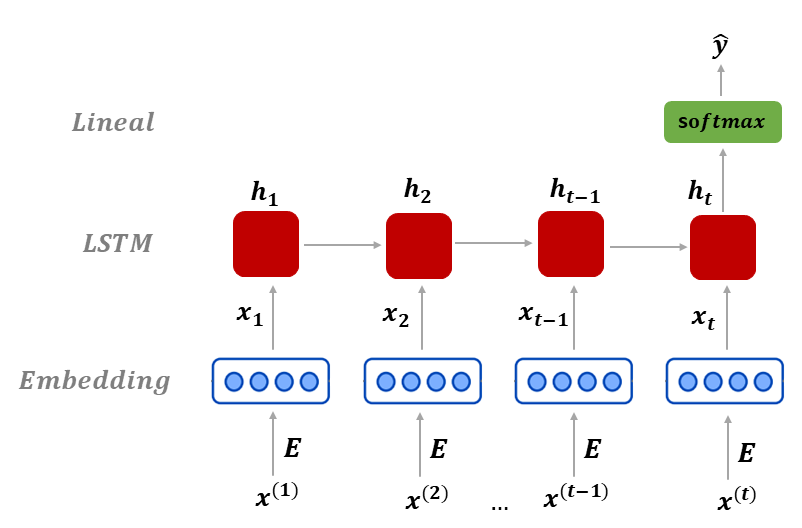
\includegraphics[angle=0, width=0.75\textwidth]{Graphics/lstm2.png} 
  \end{center}
    \caption{Arquitectura del modelo de extracción de relaciones LSTM básico}\label{lstm}
\end{figure}

Sea $S = [x^{(1)}, x^{(2)}, ..., x^{(T)}]$ la representación vectorial de una oración $S$, donde $x^{(t)}$ representa el t-ésimo \textit{token} con $(t = 1, 2, ..., T)$ y $T$, la cantidad de \textit{tokens} de la oración. El modelo puede ser definido formalmente como:

\begin{align}
  x_{t} &= Ex^{(t)} \label{lstm:emb} \\
  \nonumber \\
  i_{t} &= \sigma{(W^{(i)} x_{t} + U^{(i)}h_{t-1})} \label{lstm:ig} \\
  f_{t} &= \sigma{(W^{(f)} x_{t} + U^{(f)}h_{t-1})} \label{lstm:fg} \\
  o_{t} &= \sigma{(W^{(o)} x_{t} + U^{(o)}h_{t-1})} \label{lstm:og} \\
  \tilde{c_{t}} &= \tanh(W^{(c)} x_{t} + U^{(c)}h_{t-1}) \label{lstm:new_memory_generation} \\
  c_{t} &= f_{t}c_{t-1} + i_{t}\tilde{c_{t}} \label{lstm:cell_state} \\
  h_{t} &= o_{t}\tanh{c_{t}} \label{lstm:hidden_state} \\
  \nonumber \\
  \hat{y} &= softmax(Uh_{T} + b) \label{lstm:pred}
\end{align}

En una primera etapa (Ecuación \ref{lstm:emb}), el modelo obtiene una representación más rica semánticamente de cada uno de los \textit{tokens} que conforman una oración. Esto se logra a través de una capa de \textit{embeddings} $E$ que transforma cada \textit{token} $x^{(t)}$ en un vector $x_{t}$ $\in$ ${\mathbb{R}} ^{d}$, donde $d$ es la dimensión de los \textit{embeddings} que constituye un hiperparámetro del modelo.

En la segunda etapa (Ecuaciones \ref{lstm:ig} - \ref{lstm:hidden_state}), el modelo procesa la secuencia de \textit{tokens} para obtener una representación final de la oración. Esto se logra con la inclusión de una capa \textit{LSTM}, la cual analiza de manera secuencial cada una de las salidas $x_{t}$ de la capa de \textit{embeddings}. El centro de una red \textit{LSTM} es el funcionamiento de sus celdas, una red \textit{LSTM} tiene tantas celdas como \textit{tokens} tiene una oración. Las Ecuaciones \ref{lstm:ig} - \ref{lstm:hidden_state} describen el comportamiento de una celda de la red \textit{LSTM}. En la tabla \ref{tab:cell_state} se describe la notación empleada.

\begin{table}[!tb]
  \center \caption{Descripción de símbolos utilizados en una red \textit{LSTM}}
    \begin{center}
      \begin{tabular}{|c|l|}
        \hline
        \textbf{Símbolo} & \textbf{Significado}\\
        \hline
        $x_{t}$ & entrada a la celda \textit{LSTM} en el paso $t$ \\
        $h_{t-1}$ & salida de la celda \textit{LSTM} en el paso $t-1$ \\
        $i_{t}$ & valor de la \textit{input gate} en el paso $t$\\
        $f_{t}$	& valor de la \textit{forget gate} en el paso $t$ \\
        $o_{t}$	& valor de la \textit{output gate} en el paso $t$\\
        $\sigma$ & función sigmoidal\\
        $W^{(\alpha)}$ & pesos de $x_{t}$ en $\alpha_t$ ($\alpha = {i, f, o}$) \\
        $U^{(\alpha)}$ & pesos de $h_{t-1}$ en $\alpha_t$ ($\alpha = {i, f, o}$) \\
        $\tilde{c_{t}}$ & candidato a \textit{cell state} en el paso $t$\\
        $c_{t}$ & \textit{cell state} en el paso $t$ \\
        $h_{t}$ & salida final de la celda \textit{LSTM} en el paso $t$ \\
        $h_{T}$ & salida final de la celda \textit{LSTM} en el último paso $T$ \\
        \hline
        \end{tabular}
    \end{center}
    \label{tab:cell_state}
\end{table}

Una celda \textit{LSTM} está compuesta por tres componentes fundamentales:
\begin{itemize}
  \item La \textit{input gate}, en español "válvula de entrada", expresada en la Ecuación \ref{lstm:ig}, tiene la función de determinar qué información debe estar presente en el estado de la celda (en inglés, \textit{cell state}) representado por $c_{t}$, teniendo en cuenta la salida final de la celda anterior $h_{t-1}$.
  \item La \textit{forget gate}, en español "válvula del olvido", representada en la Ecuación \ref{lstm:fg}, tiene la función de determinar qué información es irrelevante en el estado de la celda $c_{t}$; funciona de manera análoga a la \textit{input gate}.
  \item La \textit{output gate}, en español "válvula de salida", representada en la Ecuación \ref{lstm:og}, tiene la función de determinar el nivel de activación del estado $c_{t}$ para la salida final.
\end{itemize}

En todos estos casos, se utiliza como función de activación la función sigmoide $\sigma$ con el propósito de que los valores sean positivos y se encuentren entre 0 y 1; de esa manera es sencillo interpretar la importancia de las componentes.

La Ecuación \ref{lstm:new_memory_generation}, conocida como \textit{new memory generation} o \textit{candidate cell}, calcula un estado recurrente temporal $\tilde{c_{t}}$ teniendo en cuenta la entrada $x_{t}$ y el estado anterior $h_{t-1}$. En este caso, para superar el problema de \textit{vanishing gradient}\footnote{https://towardsdatascience.com/the-vanishing-gradient-problem-69bf08b15484} se necesita una función de activación cuya segunda derivada pueda mantenerse durante un largo rango antes de llegar a cero, razón por la cual se utiliza la tangente.

En la Ecuación \ref{lstm:cell_state} se calcula el estado de la celda actual $c_{t}$ teniendo en cuenta qué debe olvidar del estado previo a través de la expresión $f_{t}*c_{t-1}$ y qué debe considerar del estado actual temporal representado en la expresión $i_{t}*\tilde{c_{t}}$. En la Ecuación \ref{lstm:hidden_state} se toma el estado de la celda $c_{t}$ y la \textit{output gate} $o_{t}$ para determinar qué información queda contenida en el estado último de la celda $h_{t}$.

Es importante destacar que los parámetros $E$, $W^{(i)}$, $W^{(f)}$, $W^{(o)}$, $W^{(c)}$, $U^{(i)}$, $U^{(f)}$, $U^{(o)}$, $U^{(c)}$ y $U$ son aprendidos durante la etapa de entrenamiento en el proceso de \textit{backpropagation}.

Las operaciones presentadas en las ecuaciones \ref{lstm:ig} - \ref{lstm:hidden_state} son ejecutadas $T$ veces, por cada uno de los \textit{tokens} que conforman una oración. Tras el análisis del último \textit{token} $T$, el estado final $h_{T}$ constituye una representación de la oración $S$. Finalmente, una capa lineal (Ecuación \ref{lstm:pred}) utiliza la representación de la oración obtenida $h_{T}$ para predecir la relación $\hat{y}$ existente en la oración. Esta salida se convierte en una distribución de probabilidades empleando la función \textit{softmax}. Esta operación, a diferencia de las ecuaciones anteriores, solo se aplica una vez al estado final $h_{T}$ de la capa \textit{LSTM}.

La sencillez arquitectónica del modelo permite que se pueda utilizar como base para la comparación con otros modelos más complejos que serán abordados a continuación.

\section{\textit{BiLSTM+Att}}\label{bilstm_t}

El tercer modelo propuesto tiene una arquitectura más compleja que el anterior consistiendo, esencialmente, en una red \textit{BiLSTM} integrada con un mecanismo de atención.

En este caso, se adiciona el uso de un modelo del lenguaje (en inglés, \textit{language model})  (\cite{mikolov-2016-fastext}) pre-entrenado en un conjunto de documentos en idioma español con el propósito de ganar riqueza semántica en la representación de la oración. Utilizar un modelo pre-entrenado ofrece la posibilidad de aprovechar el conocimiento del lenguaje contenido en la representación de las palabras (a través de los \textit{embeddings} pre-entrenados en una tarea auxiliar) en nuestra tarea específica que, en este caso, es la selección de respuestas. El modelo del lenguaje empleado es el presentado por \cite{mikolov-2016-fastext}, entrenado sobre un conjunto de artículos médicos tomados de la biblioteca electrónica \textit{Scielo}\footnote{https://scielo.isciii.es/scielo.php} tomados de \cite{2019-medical-fastext}.

Las redes recurrentes unidireccionales en general, en el análisis de una palabra, tienen en cuenta solo las palabras anteriores (o posteriores), sin embargo sería útil que al hallar la representación de una palabra se tuviera en cuenta tanto las palabras que aparecen antes como las que aparecen después en una oración. Por esta razón se decide utilizar una capa \textit{BiLSTM}, esto posibilita que en cada estado de una secuencia, la red tenga una visión completa y consecutiva de todos los estados anteriores y posteriores. Se propone la inclusión de una capa de atención pues podría ayudar al modelo a darle más peso a ciertas palabras en la oración que pueden ser determinantes en la predicción.

En la figura \ref{bilstm} se expone la arquitectura de la red correspondiente al modelo matemático que se presenta en esta sección. Seguidamente se presenta una parte de la representación formal del modelo.

\begin{figure}[!tb]
  \begin{center}
    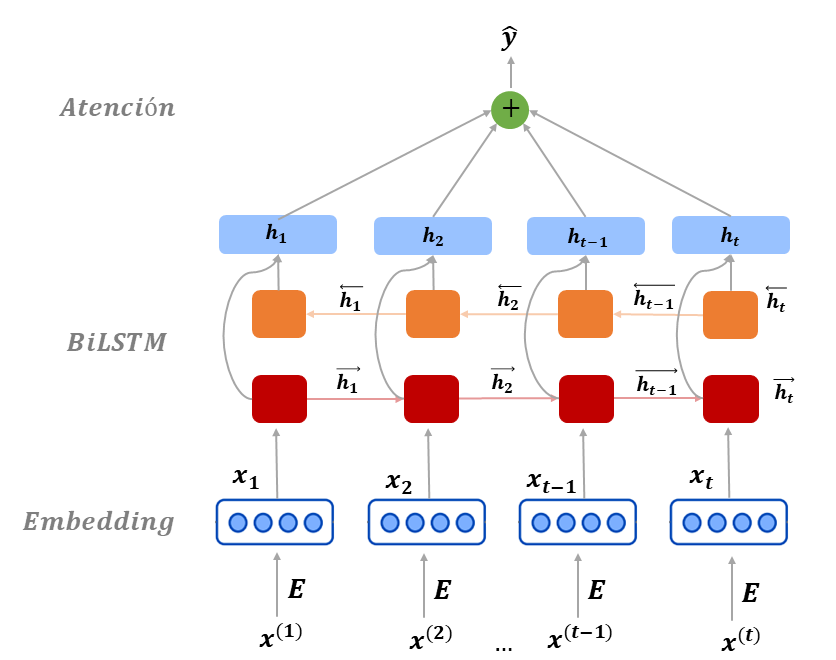
\includegraphics[angle=0, width=0.75\textwidth]{Graphics/bilstm.png}
  \end{center}
    \caption{Arquitectura del modelo de extracción de relaciones \textit{BiLSTM+Att}}\label{bilstm}
\end{figure}

Sea $S = [x^{(1)}, x^{(2)}, ..., x^{(T)}]$, donde $x^{(t)}$ representa el t-ésimo \textit{token} con $(t = 1, 2, ..., T)$ y $T$, la cantidad de \textit{tokens} de la oración $S$. El modelo puede ser definido formalmente como:

\begin{align}
  x_{t} &= Ex^{(t)} \label{bilstm:emb}\\
  \nonumber \\
  \overrightarrow{i_{t}} &= \sigma{(\overrightarrow{W^{(i)}} x_{t} + \overrightarrow{U^{(i)}}\overrightarrow{h_{t-1}})} \label{bilstm:ig} \\
  \overrightarrow{f_{t}} &= \sigma{(\overrightarrow{W^{(f)}} x_{t} + \overrightarrow{U^{(f)}}\overrightarrow{h_{t-1}})} \label{bilstm:fg} \\
  \overrightarrow{o_{t}} &= \sigma{(\overrightarrow{W^{(o)}} x_{t} + \overrightarrow{U^{(o)}}\overrightarrow{h_{t-1}})} \label{bilstm:og} \\
  \overrightarrow{\tilde{c_{t}}} &= \tanh(\overrightarrow{W^{(c)}} x_{t} + \overrightarrow{U^{(c)}}\overrightarrow{h_{t-1}}) \label{bilstm:new_memory_cell}
\end{align}

\begin{align}
  \overrightarrow{c_{t}} &= \overrightarrow{f_{t}}\overrightarrow{c_{t-1}} + \overrightarrow{i_{t}}\overrightarrow{\tilde{c_{t}}} \label{bilstm:cell_state} \\
  \overrightarrow{h_{t}} &= \overrightarrow{o_{t}}\tanh{\overrightarrow{c_{t}}} \label{bilstm:hidden_state}\\
  \nonumber \\
  \overleftarrow{i_{t}} &= \sigma{(\overleftarrow{W^{(i)}} x_{t} + \overleftarrow{U^{(i)}}\overleftarrow{h_{t+1}})} \label{bilstml:ig} \\
  \overleftarrow{f_{t}} &= \sigma{(\overleftarrow{W^{(f)}} x_{t} + \overleftarrow{U^{(f)}}\overleftarrow{h_{t+1}})} \label{bilstml:fg} \\
  \overleftarrow{o_{t}} &= \sigma{(\overleftarrow{W^{(o)}} x_{t} + \overleftarrow{U^{(o)}}\overleftarrow{h_{t+1}})} \label{bilstml:og} \\
  \overleftarrow{\tilde{c_{t}}} &= \tanh(\overleftarrow{W^{(c)}} x_{t} + \overleftarrow{U^{(c)}}\overleftarrow{h_{t+1}}) \label{bilstml:new_memory_cell} \\
  \overleftarrow{c_{t}} &= \overleftarrow{f_{t}}\overleftarrow{c_{t+1}} + \overleftarrow{i_{t}}\overleftarrow{\tilde{c_{t}}} \label{bilstml:cell_state} \\
  \overleftarrow{h_{t}} &= \overleftarrow{o_{t}}\tanh{\overleftarrow{c_{t}}} \label{bilstml:hidden_state}
\end{align}

El modelo contiene una primera capa de \textit{embeddings} pre-entrenada que transforma el \textit{word index} en una representación más rica semánticamente representada como un vector $x_{t} \in {\mathbb{R}} ^{d}$, donde $d$ es la dimensión de los \textit{embeddings} que constituye un hiperparámetro del modelo. Es importante aclarar que la Ecuación \ref{bilstm:emb} luce exactamente como la Ecuación \ref{lstm:emb} correspondiente al modelo anterior, la diferencia se encuentra en que en el modelo \textit{LSTM} los pesos de la capa de \textit{embeddings} $E$ se aprenden durante la etapa de entrenamiento, mientras que, en este caso, los pesos que se utilizan pertenecen a \textit {embeddings} pre-entrenados tomados de \cite{2019-medical-fastext} que ya contienen un conocimiento del idioma español y del dominio médico específicamente, adquirido previamente.

Una segunda capa está conformada por una red \textit{Bi-LSTM}, la cual permite tener en cuenta para el cómputo de un estado no solo las palabras anteriores sino también las siguientes. Las Ecuaciones \ref{bilstm:ig} - \ref{bilstm:hidden_state} representan la \textit{LSTM} orientada de izquierda a derecha, que comienza en el principio de la oración y concluye en el final, mientras que en las Ecuaciones \ref{bilstml:ig} - \ref{bilstml:hidden_state} representan la \textit{LSTM} orientada en sentido contrario, de derecha a izquierda. La arquitectura de la red bidireccional es muy similar a la presentada en el modelo anterior, con la diferencia que se han incluido las flechas para indicar el sentido de la red.

Las ecuaciones serán aplicadas secuencialmente a cada uno de los \textit{tokens} $x^{(t)}$ que conforman una oración $S$. En este caso, a diferencia del modelo presentado anteriormente, en lugar de utilizar solo el último estado $h_{T}$ de la red, se utilizan todos los estados intermedios $h_{t}$  $(t = 1, 2, ..., T)$. De manera que, por cada capa \textit{LSTM}, se obtiene un conjunto de estados $h_{1}, h_{2}, ..., h_{T}$.

En el caso de la red \textit{BiLSTM} se obtienen dos conjuntos de estados. Se utiliza la notación $\overrightarrow{h_{t}}$ y $\overleftarrow{h_{t}}$ como referencia al t-ésimo estado de la red izquiera-derecha y derecha-izquierda respectivamente. Por lo que, los dos conjuntos de estados intermedios se representan como $\overrightarrow{h_{1}}, \overrightarrow{h_{2}}, ... \overrightarrow{h_{T}}$ y $\overleftarrow{h_{1}}, \overleftarrow{h_{2}}, ... \overleftarrow{h_{T}}$. En el resto del modelo, en función de ganar claridad en la escritura, se utilizará $\overrightarrow{h_{t}}$ y  $\overleftarrow{h_{t}}$ para denotar los estados intermedios de forma genérica.

\begin{align}
  h_{t} &= [\overrightarrow{h_{t}} \oplus \overleftarrow{h_{t}}] \label{bilstm:concat} \\
  W &= \tanh{(IW_{a} + B)} \label{bilstm:dense} \\
  A &= sofmax(W) \label{bilstm:sig} \\
  c &= IA^{T} \label{bilstm:dot} \\
  \hat{y} &= softmax(Uc + b) \label{bilstm:pred}
\end{align}

donde $h_{t} \in {\mathbb{R}} ^{2d}$ es el resultado de concatenar $\overrightarrow{h_{t}} \in {\mathbb{R}} ^{d}$ con $\overleftarrow{h_{t}} \in {\mathbb{R}} ^{d}$ y constituye el estado definitivo de la celda $t$, expresado en la Ecuación \ref{bilstm:concat}. La salida de la capa \textit{BiLSTM} constituye entonces, un conjunto de estados $I  = {[h_{1}, h_{2}, ..., h_{T}]}$ con $I \in {\mathbb{R}}^{(T \times 1)}$.

El objetivo de incluir un mecanismo de atención es que el modelo dé mayor peso a aquellas palabras que tienen una mayor influencia en la predicción final. Intuitivamente, lo que se quiere es un vector de pesos con el mismo tamaño $T$ que la cantidad de palabras de la oración. Dicho vector debe poseer en cada componente un número positivo entre 0 y 1 que indique cuán relevante es esa palabra para la clasificación. Por esta razón, la Ecuación \ref{bilstm:dense} toma la salida de la red \textit{BiLSTM}, $I \in {\mathbb{R}}^{(T \times 1)}$, como entrada a una capa densa, donde $W_{a}$ es la matriz aprendida durante la etapa de entrenamiento, con función de activación tangente que obtiene como salida el vector de pesos no normalizado $W$. Con el objetivo de expresar los valores de $W$ en una escala entre 0 y 1 se aplica la función \textit{softmax}, como se muestra en la Ecuación \ref{bilstm:sig}, obteniendo un vector $A$ distribuido probabilísticamente cuyas componentes representan los pesos de atención. En la Ecuación \ref{bilstm:dot} se combina el vector de pesos de atención $A$ con la salida de la capa \textit{BiLSTM} dando como resultado un vector $c$, conocido como vector contexto, que constituye la representación final de la oración. Finalmente, una capa lineal utiliza la representación de la oración obtenida $c$ para predecir la relación $\hat{y}$ existente en la oración. Esta salida se convierte en una distribución de probabilidades empleando la función \textit{softmax}.

\section{\textit{Transfer Learning} basado en BERT}\label{bert_t}

\cite{2018-devlin-bert} plantea que el uso de BERT en el enfoque \textit{fine tuning} obtiene nuevos resultados en el estado del arte en varias tareas de procesamiento del lenguaje natural, entre ellas, el reconocimiento de entidades nombradas y los sistemas pregunta/respuesta.

La diferencia con otros modelos de representación del lenguaje, en cuanto a arquitectura, es que BERT está basado en un \textit{Transformer} bidireccional. En el artículo de \cite{2018-devlin-bert} no se detalla la arquitectura del modelo \textit{Transformer}. Otra diferencia es que modifica la tarea tradicional de \textit{language modeling} sobre la que se entrena introduciendo nuevas tareas. La primera tarea introducida recibe el nombre de \textit{masked language model} y consiste en ocultar palabras aleatorias en un texto y predecir, teniendo en cuenta el contexto, el \textit{token} que corresponde a la posición oculta, mientras que la segunda tarea consiste en, dada una oración en un texto, predecir la oración siguiente.

Los autores de BERT señalan como principal contribución la demostración de la efectividad del pre-entrenamiento bidireccional en la representación del lenguaje sobre las arquitecturas unidireccionales utilizadas hasta ese momento y, además, plantean que con el uso de esta nueva representación se puede reducir la complejidad de la arquitectura del modelo y aún así, obtener mejores resultados.

En esta tesis se propone un modelo que hace uso del modelo de lenguaje aprendido utilizando BERT e incorpora un modelo de predicción simple. La propuesta tiene como objetivo comprobar si los aportes de BERT se pueden extender al idioma español y, específicamente, a la tarea de extracción de relaciones semánticas entre entidades.

\section{QA LSTM}

\section{QA LSTM + CNN}

\section{QA BERT}

\subsection{Especificidad del preprocesamiento}

Con el objetivo de transformar una oración en un vector computacionalmente interpretable, se propuso un preprocesamiento que fue aplicado a los modelos de aprendizaje presentados. Sin embargo, en el caso de BERT, las oraciones no pueden ser traducidas a vectores numéricos de la misma forma que se hizo en las propuestas anteriores, sino que BERT requiere un formato diferente. Con el fin de obtener los resultados esperados, el corpus original siempre debe ser modificado en función de las pautas planteadas por los autores en \cite{2018-devlin-bert}.

BERT define los siguientes \textit{tokens} especiales para la representación de una oración. Dichos \textit{tokens} reciben una interpretación diferente en la etapa de entrenamiento.
\begin{itemize}
  \item \textbf{[CLS]}: Indica el inicio de una oración
  \item \textbf{[SEP]}: Indica el fin de una oración
  \item \textbf{[MASK]}: Se utiliza para denotar \textit{tokens} que deben ser ignorados por el modelo
\end{itemize}

BERT no acepta secuencias de tamaño variable por lo que se recurre a la estrategia de \textit{padding}, en la que se establece un tamaño máximo. Las oraciones que tienen una cantidad menor de \textit{tokens} son completadas con el \textit{token} especial \textbf{[MASK]}, para indicar que esas posiciones deben ser ignoradas.

\section{Implementación}





\chapter{Resultados}\label{chapter:results}

A lo largo de esta tesis se han concebido y diseñado varios modelos para resolver la tarea de selección de respuestas a partir de un corpus previamente construido. En el presente capítulo, se expone un conjunto de experimentos desarrollados con el propósito de medir el desempeño de los modelos propuestos en dicha tarea.

\section{Medidas de Evaluación}

Con el propósito de medir la eficacia de los modelos propuestos es necesario la aplicación de medidas estándares utilizadas en el paradigma del aprendizaje automático. Para la evaluación de los modelos propuestos se utiliza como métrica la \textbf{Exactitud}. Asimismo, teniendo en cuenta el escenario también se utiliza como métrica de evaluación la puntuación característica de estos exámenes y que es la empleada realmente para calificar los exámenes cada año.

Supongamos que estamos en presencia de un problema de clasificación binario cualquiera, donde solo existen dos clases que llamaremos $C^{+}$ y $C^{-}$. Los posibles tipos de respuestas de un modelo se definen como:

\begin{description}
  \item \textbf{\textit{True Positive} (TP)}: Un ejemplo se clasifica en \textbf{TP}, traducido al español como Verdadero Positivo, cuando la clase predicha coincide con la clase correcta $C^{+}$. En este caso, la predicción hecha fue correcta.
  \item \textbf{\textit{False Positive} (FP)}: Un ejemplo se clasifica en \textbf{FP}, en español Falso Positivo, cuando el valor predicho es $C^{+}$, sin embargo su valor correcto es $C^{-}$. En este caso, el modelo hizo una predicción equivocada.
  \item \textbf{\textit{False Negative} (FN)}: Una instancia se clasifica en \textbf{FN}, en español Falso Negativo, cuando el valor predicho es $C^{-}$, sin embargo su clase correcta es $C^{+}$. En este caso, como en el anterior, el modelo hizo una predicción incorrecta.
  \item \textbf{\textit{True Negative} (TN)}: Una instancia se clasifica en \textbf{TN}, en español, Verdadero Negativo, cuando la clase predicha corresponde con la clase correcta $C^{-}$, lo que implica que el modelo hizo una predicción acertada.
\end{description}

Estos tipos de respuestas se representan visualmente en la matriz de confusión que se muestra en la tabla \ref{tab:confusion}.

\begin{table}[h!]
  \caption{Matriz de confusión para un problema de clasificación binario}
  \begin{center}
    \begin{tabular}{ccc|cc|cc}
        & Valor Correcto/Valor Predicho &    & $\mathbf{C}^{\boldsymbol{+}}$ & & $\mathbf{C}^{\boldsymbol{-}}$  \\
        \hline
        & $\mathbf{C}^{\boldsymbol{+}}$ &   & TP & & FN  \\
        \hline
        & $\mathbf{C}^{\boldsymbol{-}}$ &   & FP & & TN  \\
    \end{tabular}
  \end{center}
  \label{tab:confusion}
\end{table}

La \textbf{Exactitud} (en inglés \textit{Accuracy}) se interpreta como la razón entre las predicciones correctas ($TP + TN$) y la cantidad total de instancias que analizó el modelo. Se computa sobre los resultados generales del modelo y se define como:

\begin{equation}
  E = \frac{TP + TN}{\textit{Total de Ejemplos}}
\end{equation}

La métrica estándar para calificar este tipo de exámenes consiste en sumar tres puntos si la respuesta está correcta y -1 si es incorrecta.

\section{Técnicas de remuestreo}

En esta sección se detalla el proceso de entrenamiento de los modelos propuestos anteriormente. 

Dado que una instancia del conjunto original se convierte en varios ejemplos diferentes, una por cada posible respuesta y que solo una de las respuestas es correcta, el conjunto de datos resultante del procesamiento de texto es un conjunto desbalanceado. Por una instancia positiva pueden aparecer al menos 3 instancias negativas.

Un conjunto de datos desbalanceado es el problema en el que los datos que pertenecen a una clase son significativamente más altos o más bajos que los que pertenecen a otras clases, como es el caso. La mayoría de los algoritmos de clasificación ML/DL no están equipados para manejar clases desequilibradas y tienden a inclinarse hacia las clases mayoritarias.

Para enfrentar este problema se han implementado varias técnicas de remuestreo cuyo objetivo es equilibrar la cantidad de muestras en cada una de las clases. La idea más sencilla para balancear un conjunto de datos es añadiendo muestras de la clase minoritaria o eliminando de la clase mayoritaria, sin embargo, estás técnicas tienen riesgo de \textit{overfitting} y \textit{underfitting} respectivamente. En la práctica resultan más efectivas técnicas avanzadas como SMOTE (del inglés, \textit{Synthetic Minority Over-sampling Technique}) que crean datos sintéticos de la case minoritaria. Sin embargo, SMOTE no se desempeña bien en el ámbito de los datos textuales por la alta dimensionalidad de los vectores que se obtienen a partir de texto.

Teniendo en cuenta esto, se han implementado las siguientes técnicas de remuestreo:

\begin{itemize}
  \item \textit{Random Undersampling}: Este algoritmo consiste en eliminar del conjunto de datos transformados instancias negativas de manera aleatoria hasta igualar la cantidad de instancias positivas y negativas.
  \item \textit{Random oversampling}: Este proceso es muy similar al anterior desde el punto de vista de la aleatoriedad pero adiciona instancias positivas al \textit{dataset} hasta igualar la cantidad de instancias de cada etiqueta.
  \item \textit{Mixed oversampling}: El objetivo de esta técnica es reproducir el comportamiento de los algoritmos de generación sintética de datos. El concepto también es similar a \textit{Data Augmentation}, común en el procesamiento de imágenes, que implica la creación de nuevas instancias aplicando transformaciones (como rotar, trasladar, escalar, entre otras) las del conjunto de datos original. En este caso, para generar texto a partir de las oraciones originales se recurre a la traducción y al reemplazamiento por sinónimos. El algoritmo de traducción toma una oración y la traduce al idioma inglés, del inglés al alemán y luego, nuevamente al castellano. Se introduce un idioma intermedio para lograr una mayor diferencia entre la oración original y la resultante. Esto podría resultar contraproducente pues puede cambiar el sentido de la oración original, lo cual se verá en la evaluación de los modelos. Por otra parte, la otra técnica consiste en a partir de una oración obtener otra compuesta por las palabras más parecidas a cada una de las palabras de la oración original. Las palabras más similares a un témino dado se han determinado a partir del uso de sus \textit{word embeddings}. En este caso, se han utilizado \textit{embeddings} obtenidos aplicando el algoritmo Fasttext sobre el \textit{Spanish Billion Word Corpus}\footnote{http://crscardellino.github.io/SBWCE/} descargado de \cite{spanish-word-embeddings}. 
\end{itemize}

En las secciones posteriores se muestran los resultados de los modelos propuestos utilizando como entrenamiento las diferentes técnicas de remuestreo.

\section{Entrenamiento}

Además de los modelos de aprendizaje profundo detallados en el capítulo anterior, se implementa un modelo de regresión logística, que por su simplicidad, es utilizado como \textit{baseline} supervisado, al no existir soluciones anteriores que utilicen este tipo de aprendizaje.

La métrica utilizada por los autores del \textit{dataset} es la \textit{Exactitud} y la cantidad de puntos, ambos a nivel de examen. Lo que quiere decir que, aunque los enfoques supervisados implementados interpretan el problema como una tarea de clasificación binaria y se puede calcular la exactitud sobre el conjunto de datos transformado, no se utilizará esta forma para expresar los resultados finales en aras de poder comparar los resultados con los ya existentes en la literatura.

Por esta razón, esta sección se centra en el proceso de entrenamiento y el análisis de los resultados sobre el conjunto de datos transformado. Mientras que la próxima sección se centra en el cálculo de la \textbf{Exactitud} sobre los datos originales y presenta los resultados finales comparables con los ya existentes.

Para analizar el proceso de entrenamiento nos centraremos en estudiar la evolución de los algoritmos implementados sobre el conjunto de datos de entrenamiento resultante de aplicar la técnica de remuestreo \textit{Random Oversampling}. 

El objetivo de este análisis es comrpobar si la transformación a un problema de clasificación binario en este escenario es válida y si se corresponden con los resultados finales sobre el conjunto original.

En la Figura \ref{loss_lreg} se muestra la evolución de la función de pérdida durante el entrenamiento del modelo de Regresión Logística, mientras que en la Figura \ref{loss_all} del resto de los modelos supervisados, exceptuando el basado en BERT. Este último no se incluyó porque la cantidad de epochs utilizada es muy pequeña. La función de pérdida utilizada fue \textit{Binary Cross Entropy}.

\begin{figure}[!tb]
  \begin{center}
    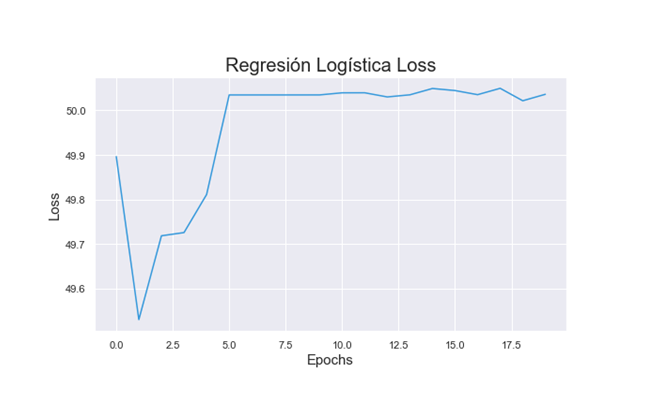
\includegraphics[angle=0, width=1\textwidth]{Graphics/loss_lreg.png}
  \end{center}
    \caption{Función de pérdida del modelo Regresión Logística durante el entrenamiento}\label{loss_lreg}
\end{figure}

\begin{figure}[!tb]
  \begin{center}
    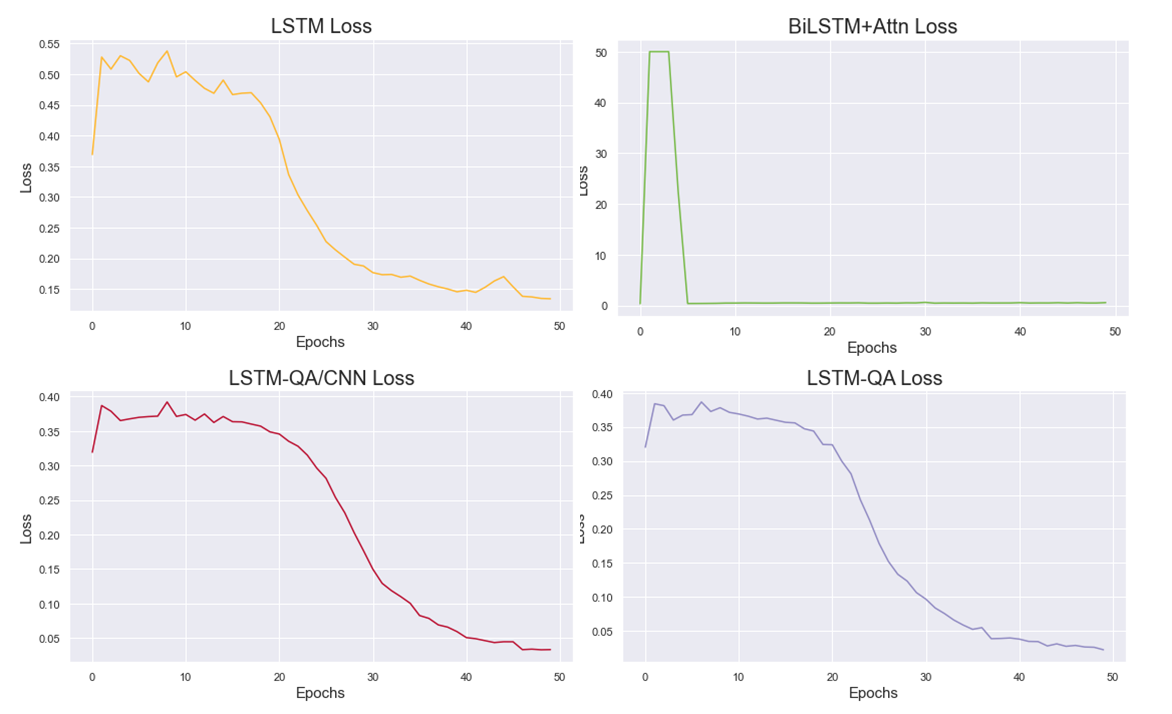
\includegraphics[angle=0, width=1\textwidth]{Graphics/loss_all.png}
  \end{center}
    \caption{Función de pérdida de los modelos supervisados durante el entrenamiento}\label{loss_all}
\end{figure}

Se puede observar que el modelo de regresión no logra minimizar la función de pérdida a partir de los datos de entrenamiento, por lo que se puede pensar que este modelo no tiene la capacidad o los datos de entrenamiento no son son suficientes, sufriendo de \textit{underfitting}. También se puede notar en la segunda imagen que el modelo BiLSTM+Attn aunque logra minimizar la pérdida, se queda por encima del resto de los modelos que logran minimizar a valores cercanos a 0,05. A partir del comportamiento de esta función, se espera que los modelos LSTM, LSTM-QA y LSTM-QA/CNN sean los que mejor desempeño alcancen.

En este caso, como estamos en presencia de conjuntos de datos imbalanceados, aunque se balanceó el de entrenamiento, el de validación y test no se modificaron en ese sentido, no es recomendable utilizar la exactitud como métrica de evaluación. Por esta razón, se visualiza la matriz de confusión para cada uno de los modelos entrenados.

En la Figura \ref{dev_cm} se muestra la matriz de confusión de los modelos sobre el conjunto de validación, mientras que la Figura \ref{test_cm} corresponde a los resultados sobre le conjunto de test.

\begin{figure}[!tb]
  \begin{center}
    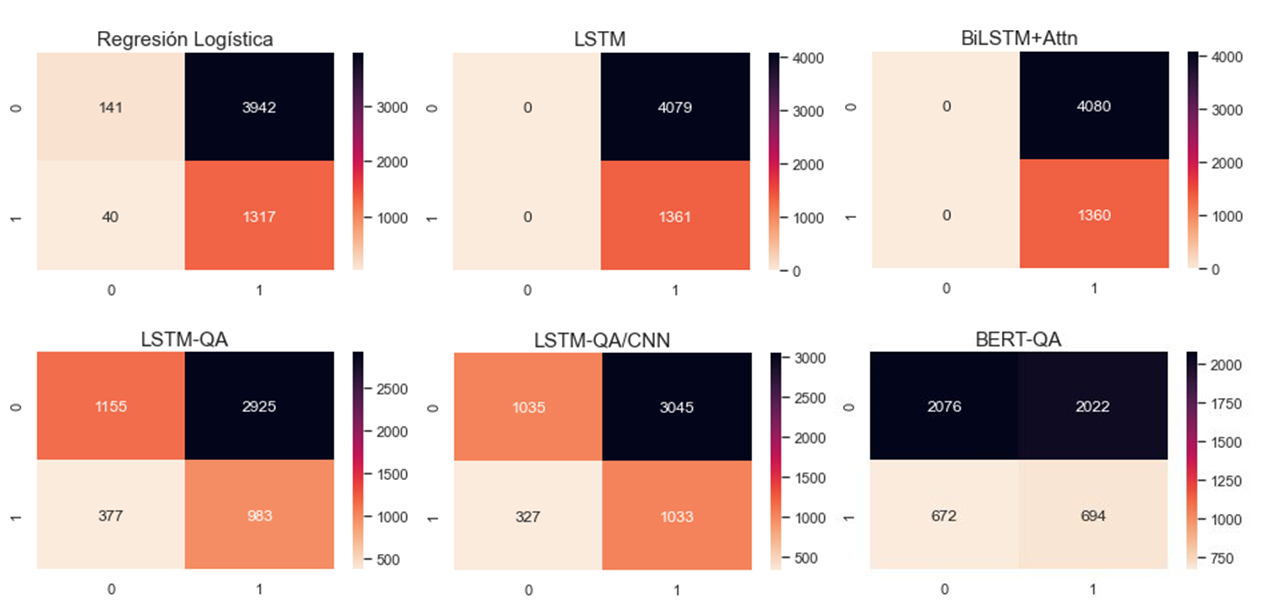
\includegraphics[angle=0, width=1\textwidth]{Graphics/dev_cm.png}
  \end{center}
    \caption{Matriz de confusión DEV}\label{dev_cm}
\end{figure}

\begin{figure}[!ht]
  \begin{center}
    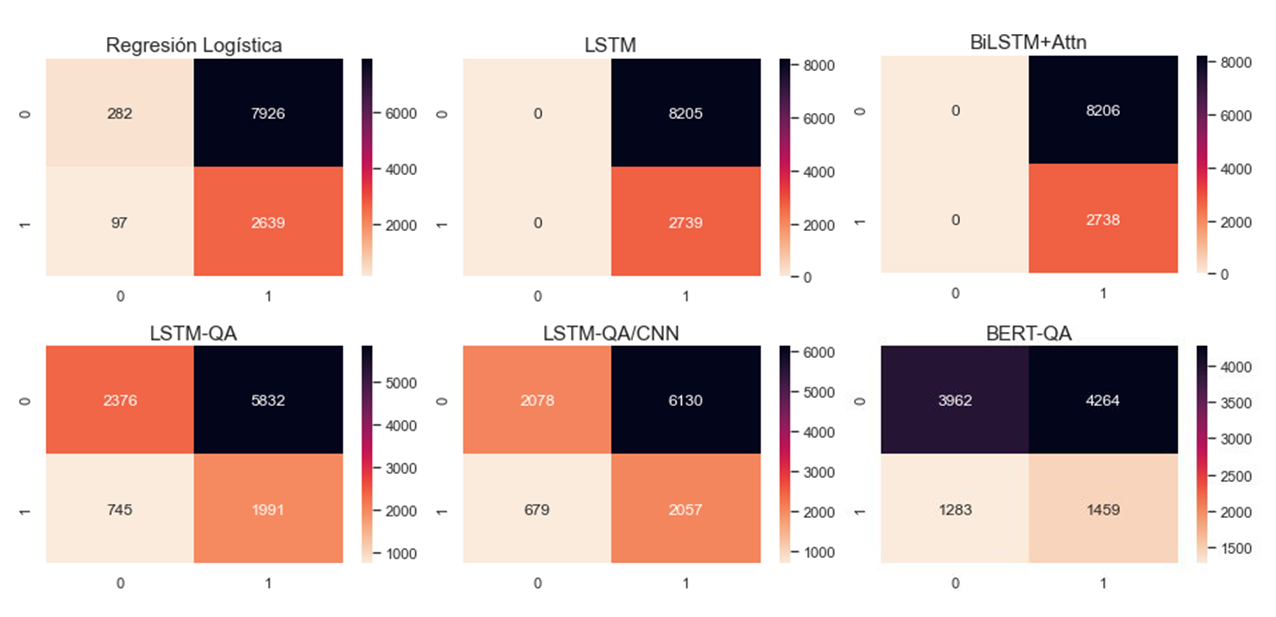
\includegraphics[angle=0, width=1\textwidth]{Graphics/test_cm.png}
  \end{center}
    \caption{Matriz de confusión TEST}\label{test_cm}
\end{figure}

En la Figura \ref{dev_cm} se puede notar como el algoritmo de regresión a pesar de no haber logrado optimizar la función de pérdida, da algunos resultados correctos. Por otra parte, es notable que LSTM y BiLSTM predicen siempre la clase positiva. Los últimos tres modelos son los que más han logrado aprender del conjunto de entrenamiento, sin embargo también se puede notar una tendencia a la clase positiva. Este comportamiento es muy similar en el conjunto de test como se puede observar en la Figura \ref{test_cm}. Predecir la clase postiva significa que los modelos dan una gran relevancia a la mayoría de las posibles respuestas. Sin embargo, esto necesariamente no tiene por qué ser negativo al ser aplicado en el problema original, pues en ese caso se toma como correcta solo la posible respuesta con mayor relevancia.

Tras este análisis se puede concluir que si bien algunos de los algoritmos han logrado aprender de los datos, especialmente los que incluyen el enfoque de recuperación de información, el desempeño no ha sido muy bueno de manera general, aunque era esperado dada los resultados tan bajos que se han obtenido también en la literatura. Esto puede tener varias causas: los algoritmos sufren de \textit{underfitting} y necesitan más entrenamiento sobre los mismos datos o necesitan más datos. El proceso de entrenamiento durante la experimentación se detuvo cuando se observó una estabilidad en la pérdida, por lo que existe una mayor posibilidad de que los datos no sean suficientes dada la complejidad del problema.

En la siguiente sección nos centraremos en exponer los resultados finales sobre el conjunto original.

\section{Evaluación}

Como se mencionó anteriormente, las preguntas del conjuntos de datos están separadas por categorías. Tras el análisis descriptivo inicial, se pudo notar que las palabrás más comunes al separar los datos diferían según la temática, o sea, el vocabulario varía de acuerdo al dominio. Por esta razón, se decide entrenar y evaluar los modelos tanto en el conjunto de datos completo, como en los subconjuntos resultantes de filtrar por materia.

La métrica utilizada por los autores del \textit{dataset} es la \textit{Exactitud} y la cantidad de puntos, ambos a nivel de examen. Lo que quiere decir que, aunque los enfoques supervisados implementados interpretan el problema como una tarea de clasificación binaria y se puede calcular la exactitud sobre el conjunto de datos transformado, no se utilizará esta forma en aras de poder comparar los resultados con los ya existentes en la literatura. 

De manera que, la métrica \textbf{Exactitud} no se computará sobre el conjunto transformado a binario, sino sobre los exámenes originales. Por lo tanto, una instancia se considera correcta si la pregunta como un todo fue respondida correctamente y no si cada una de las respuestas fueron clasificadas en positivo o negativo correctamente. La \textbf{Exactitud}, además, se considera adecuada ya que las clases en el problema actual (pregunta respondida correctamente o incorrectamente) tienen el mismo pero.

Dado que los modelos supervisados anteriores en su mayoría aplican la función sigmoide en la última capa, devuelven un número entre 0 y 1, que indica cuán relevante es la posible respuesta a la pregunta. Dada una pregunta del conjunto de datos original con sus posibles respuestas, cada par se transforma en una instancia vectorizada y se da como entrada al modelo de aprendizaje. La salida del modelo para cada una de las posibles respuestas es organizada y se elige como respuesta correcta la de mayor relevancia.

A continuación, se presentan los resultados alcanzados en este trabajo. Inicialmente se presentan los resultados alcanzados por categorías y posteriormente en el conjunto de datos general.

\subsection{Evaluación por categorías}

En esta sección, se analizan los resultados de aplicar las métricas antes mencionadas sobre el conjunto de evaluación obteniendo un conjunto de valores finales y concluyentes para cada modelo, de manera que se puedan comparar con los resultados actuales. El conjunto de validación está compuesto solamente por 6 exámenes, uno de cada categoría, mientras que el conjunto de evaluación está confomado por 12, 2 de cada rama.

En la Tabla \ref{comparison_points} se presentan los resultados obtenidos en función de la cantidad de puntos por todos los modelos implementados, teniendo en cuenta las categorías. Asimismo en la Tabla \ref{comparison_accuracy}, se comparan en función de la exactitud. Adicionalmente, en ambos casos, en las líneas inferiores se incluyen las métricas reportadas en \cite{2019-head-qa} sobre el conjunto de datos en español. 

Las columnas de la tabla corresponden al nombre del modelo, el método de remuestreo aplicado sobre el conjunto de entrenamiento y los nombre de los exámenes de acuerdo a la categoría: Biología (MIR), Enfermería (EIR), Farmacología (FIR), Medicina (MIR), Psicología (PIR) y Química (QIR). 

\begin{table}[!ht]
  \begin{center}
    \caption{Comparación de los modelos por categorías por Puntos}
    \begin{tabular}{l|c|c|c|c|c|c|c}
      \textbf{Modelo} & \textbf{Entrenamiento} & \textbf{BIR} & \textbf{EIR} & \textbf{FIR} & \textbf{MIR} & \textbf{PIR} & \textbf{QIR}\\
      \hline
      Regresión Logística & \textit{Oversampled} & -3 & 7 & -9 & \textcolor{red}{469} & -8 & -7 \\
      LSTM & \textit{Oversampled} & \textbf{43} & 23 & -17 & \textcolor{red}{320} & 9 & 51\\
      BiLSTM+Attn & \textit{Oversampled} & -22 & -6 & -37 & \textcolor{red}{342} & -8 & -9\\
      QA-LSTM & \textit{Oversampled} & 41 & 17 & -3 & -4 & 13 & -5\\
      QA-LSTM/CNN & \textit{Oversampled} & -2 & -16 & -1 & -18 & 17 & 21\\

      Regresión Logística & \textit{Mixed} & 3 & -6 & -9 & \textcolor{red}{461} & -8 & -13\\
      LSTM & \textit{Mixed} & 27 & 19 & \textbf{24} & \textcolor{red}{327} & -2 & -65\\
      BiLSTM+Attn & \textit{Mixed} & -3 & -6 & -13 & \textcolor{red}{323} & -8 & -9 \\
      QA-LSTM & \textit{Mixed} & 7 & 7 & -11 & 47 & -2 & -45 \\
      QA-LSTM/CNN & \textit{Mixed} & -15 & 1 & 6 & 35 & 29 & \textbf{51} \\

      QA-BERT & \textit{Undersampled} & 38 & \textbf{25} & 3 & 41 & \textbf{49} & -26 \\
      Sim-BERT & \textit{No} & -33 & -4 & -40 & 17 & -26 & 7 \\
      \hline
      RANDOM & - & -7 & 2.5 & -10,5 & -17,5 & 26,5 & 25 \\
      $BLIND_3$ & - & 9 & 44.5 & 19,5 & 22,5 & -1,5 & 25 \\
      $LENGTH$ & - & 67 & 70,5 & 47,5 & 18,5 & 50,5 & 47 \\
      $IR$ & - & 105 & 100,5 & 139,5 & 12,5 & 98,5 & 103,5 \\
    \end{tabular}
  \end{center}
  \label{comparison_points}
\end{table}

\begin{table}[!tb]
  \begin{center}
    \caption{Comparación de los modelos por categorías por Exactitud}
    \begin{tabular}{l|c|c|c|c|c|c|c}
      \textbf{Modelo} & \textbf{Entrenamiento} & \textbf{BIR} & \textbf{EIR} & \textbf{FIR} & \textbf{MIR} & \textbf{PIR} & \textbf{QIR}\\
      \hline

      Regresión Logística & \textit{Oversampled} & 0,25 & 0,26 & 0,24 & \textcolor{red}{0,76} & 0,24 & 0,24 \\
      LSTM & \textit{Oversampled} & \textbf{0,30} & \textbf{0,27} & 0,23 & \textcolor{red}{0,60} & 0,26 & \textbf{0,31}\\
      BiLSTM+Attn & \textit{Oversampled} & 0,23 & 0,24 & 0,21 & \textcolor{red}{0,62} & 0,24 & 0,24\\
      QA-LSTM & \textit{Oversampled} & 0,25 & \textbf{0,27} & 0,25 & 0,24 & 0,26 & 0,24\\
      QA-LSTM/CNN & \textit{Oversampled} & 0,29 & 0,23 & 0,25 & 0,23 & 0,27 & 0,27\\

      Regresión Logística & \textit{Mixed} & 0,25 & 0,24 & 0,24 & \textcolor{red}{0,76} & 0,24 & 0,23\\
      LSTM & \textit{Mixed} & 0,28 & \textbf{0,27} & \textbf{0,28} & \textcolor{red}{0,60} & 0,25 & 0,32\\
      BiLSTM+Attn & \textit{Mixed} & 0,25 & 0,24 & 0,24 & \textcolor{red}{0,60} & 0,24 & 0,24 \\
      QA-LSTM & \textit{Mixed} & 0,26 & \textbf{0,27} & 0,24 & 0,30 & 0,25 & 0,20 \\
      QA-LSTM/CNN & \textit{Mixed} & 0,23 & 0,25 & 0,26 & 0,29 & 0,28 & \textbf{0,31} \\

      QA-BERT & \textit{Undersampled} & 0,27 & 0,26 & 0,25 & 0,27 & \textbf{0,28} & 0,24\\
      Sim-BERT & \textit{No} & 0,21 & 0,25 & 0,21 & 0,27 & 0,22 & 0,26\\
      \hline
      $RANDOM$ & - & 0,24 & 0,25 & 0,24 & 0,23 & 0,28 & 0,28 \\
      $BLIND_3$ & - & 0,26 & 0,29 & 0,27 & 0,27 & 0,24 & 0,27 \\
      $LENGTH$ & - & 0,32 & 0,32 & 0,30 & 0,27 & 0,30 & 0,30 \\
      $IR$ & - & 0,36 & 0,36 & 0,40 & 0,26 & 0,36 & 0,36 \\

    \end{tabular}
  \end{center}
  \label{comparison_accuracy}
\end{table}

Los modelos incluidos en la parte inferior de la tabla consisten en:
\begin{itemize}
  \item $RANDOM$: Seleccionar una respuesta de manera aleatoria.
  \item $BLIND_3$: Seleccionar siempre la tercera opción.
  \item $LENGTH$: Seleccionar la respuesta más larga.
  \item $IR$: Modelo de RI implementado en \cite{2019-head-qa} que utiliza como corpus artículos de Wikipedia.
\end{itemize}

Al analizar los resultados obtenidos en función de la cantidad de puntos, se puede notar que los algoritmos supervisados si bien alcanzan resultados superiores al modelo aleatorio la mayoría de ellos, no superan al modelo basado en recuperación de información. Los modelos que más baja puntuación alcanzan son el de regresión logística y el modelo no supervisado construido sobre BERT.
Tras el análisis anterior de los modelos durante la etapa de entrenamiento, el comportamiento del regresor era esperado. Por otra parte, el fallo del modelo BERT-SIM reafirma que un simple \textit{matching} o coincidencia entre las palabras de la pregunta y la respuesta no es suficientes para resolver este problema.

Los resultados en función de exactitud reflejan un comportamiento muy similar. Los modelos que mejor desempeño han alcanzado son el LSTM, QA-LSTM y QA-BERT.

\subsection{Evaluación general}

En esta sección se exponen los resultados tras entrenar y evaluar los modelos sobre todo el conjunto de datos, sin tener en cuenta las materias de cada pregunta. En este caso, solamente se exponen los resultados alcanzados por nuestros modelos, pues en el artículo \cite{2019-head-qa} no se desarrollaron modelos siguiendo este enfoque. 

En la Tabla \ref{comparison_points_general} se presentan los resultados obtenidos en función de la cantidad de puntos por todos los modelos implementados. De manera análoga, en la Tabla \ref{comparison_acc_general} se muestra en función de la exactitud. En cada caso se muestras las puntuaciones media y máximas obtenidas.

\begin{table}[!tb]
  \begin{center}
    \caption{Comparación general por cantidad de puntos TEST}
    \begin{tabular}{l|c|c|c}
      \textbf{Modelo} & \textbf{Entrenamiento} & \textbf{Media Pts.} & \textbf{Max Pts.}\\
      \hline
      Regresión Logística & Desbalanceado & -8 & 29 \\
      LSTM & Desbalanceado & 1 & 37 \\
      BiLSTM+Attn & Desbalanceado & 15 & 93 \\
      QA-LSTM & Desbalanceado & 15 & 74 \\
      QA-LSTM/CNN & Desbalanceado & 11 & 36 \\

      Regresión Logística & \textit{Oversampled} & -5 & 37 \\
      LSTM & \textit{Oversampled} & 2 & 56 \\
      BiLSTM+Attn & \textit{Oversampled} & -2 & 21 \\
      QA-LSTM & \textit{Oversampled} & 9 & 45 \\
      QA-LSTM/CNN & \textit{Oversampled} & 7 & 61 \\

      Regresión Logística & \textit{Mixed} & -9 & 21 \\
      LSTM & \textit{Mixed} & 11 & 39 \\
      BiLSTM+Attn & \textit{Mixed} & -3 & 40 \\
      QA-LSTM & \textit{Mixed} & \textbf{23} & \textbf{101} \\
      QA-LSTM/CNN & \textit{Mixed} & 4 & 49 \\

      QA-BERT & \textit{Undersampled} & 3 & 41 \\
      Sim-BERT & \textit{No} & -13 & 29 \\
    \end{tabular}
  \end{center}
  \label{comparison_points_general}
\end{table}

\begin{table}[!tb]
  \begin{center}
    \caption{Comparación general por cantidad de Exactitud TEST}
    \begin{tabular}{l|c|c|c}
      \textbf{Modelo} & \textbf{Entrenamiento} & \textbf{Media Exact.} & \textbf{Max Exact.}\\
      \hline
      Regresión Logística & Desbalanceado & 0, 24 & 0,28\\
      LSTM & Desbalanceado & 0,25 & 0,29 \\
      BiLSTM+Attn & Desbalanceado & \textbf{0,27} & \textbf{0,35} \\
      QA-LSTM & Desbalanceado & 0,26 & 0,33 \\
      QA-LSTM/CNN & Desbalanceado & 0,26 & 0,29 \\

      Regresión Logística & \textit{Oversampled} & 0.24 & 0,29 \\
      LSTM & \textit{Oversampled} & 0,25 & 0,31 \\
      BiLSTM+Attn & \textit{Oversampled} & 0,25 & 0,27 \\
      QA-LSTM & \textit{Oversampled} & 0,26 & 0,30 \\
      QA-LSTM/CNN & \textit{Oversampled} & 0,26 & 0,32 \\

      Regresión Logística & \textit{Mixed} & 0,24 & 0,27 \\
      LSTM & \textit{Mixed} & 0,26 & 0,29 \\
      BiLSTM+Attn & \textit{Mixed} & 0,25 & 0,29 \\
      QA-LSTM & \textit{Mixed} & \textbf{0,27} & \textbf{0,36} \\
      QA-LSTM/CNN & \textit{Mixed} & 0,25 & 0,30 \\

      QA-BERT & \textit{Undersampled} & 0,25 & 0,30 \\
      Sim-BERT & \textit{No} & 0,23 & 0,28 \\
      
    \end{tabular}
  \end{center}
  \label{comparison_acc_general}
\end{table}

Nuevamente los modelos que menor desempeño muestran son el regresor logístico y BERT-SIM. Mientras que el que mayor puntuación alcanza es LSTM-QA cuando fue entrenado con el conjunto balanceado empleando el algoritmo \textit{Mixed Oversampling}. Se puede notar que la media de las puntuaciones al entrenar con todos los datos es muy similar a la alcanzada por los modelos independientes. Mientras que la puntuación máxima en algunos casos muestra un incremento.

Sin embargo, se debe tener en cuenta que el conjunto de datos de evaluación consta de 12 exámenes distribuidos en las 6 categorías y el de validación, con solo 6. Por esta razón, no se considera que este \textit{dataset} esté preparado aún para ser utilizado por algoritmos supervisados. Si bien es cierto que la cantidad de preguntas es grande, la probabilidad de que una pregunta se parezca a preguntas de años anteriores es baja cuando solo se cuenta con un histórico de alrededor de 5 años, teniendo en cuenta que cada examen tiene entre 200 y 250 preguntas y que los exámenes están separados por categorías.

De manera general, se puede afirmar que no hay grandes diferencias en los resultados en función de los datos de entrenamiento y las técnicas de remuestreo utilizadas. 

Los algoritmos de clasificación, a diferencia de los algoritmos de regresión, durante el entrenamiento minimizan una función de pérdida seleccionada y no directamente, la exactitud de los modelos, aunque ambas estén relaciondas. De manera que, el desempeño de un modelo, depende en gran medida de la función de pérdida seleccionada. La autora considera que una función de pérdida diseñada para maximizar la importancia de una respuesta correcta y penalizar una incorrecta podrá ofrecer notables ventajas y mejorar el desempeño de los algoritmos supervisados. 

\section{Discusión de los resultados}

Tras el análisis de los resultados se puede afirmar que el conocimiento adquirido por los modelos durante la etapa de entrenamiento es válido y puede ser utilizado para la selección de respuestas. Los modelos supervisados no mostraron un desempeño superior a los modelos del estado del arte sobre este conjunto de datos, pero tampoco obtuvieron resultados muy por debajo. Sin embargo y aunque los resultados son comparables con los modelos previamente existentes, continúan estando muy lejos de las puntuaciones alcanzadas por humanos. Teniendo en cuenta que en el año 2016 la media de las 10 mejores notas según \cite{2019-head-qa} está alrededor de los 600 puntos y las notas de corte cercanas a los 200, los modelos automáticos aún están lejos de resolver este problema.

Los modelos han demostrado que no tienen la capacidad de resolver este problema sobre este conjunto de datos. Dada la complejidad del problema en cuestión, la cantidad de datos no es suficiente para construir un modelo robusto basado solamente en aprendizaje supervisado. 

\backmatter

\chapter*{Conclusiones}\label{chapter:conclusion}
\addcontentsline{toc}{chapter}{Conclusiones}
\bibliographystyle{apalike}
\bibliography{Bibliography}


\end{document}